\subsection{Questions, evidence, and setup}
The evaluation asks four separate questions. First, which structures do the
verified optimization passes remove or simplify? Second, what size and timing
cost does conversion to conjunctive guards and invariants add? Third, do the
packaged system checks behave as intended? Fourth, does optimization affect a
matched downstream check? Internal output shape is a Rocq theorem; external
checker verdicts and resource use are experimental evidence. The matched
TChecker cases below show unchanged exploration on systems whose exported
models are byte-identical before and after optimization; they do not establish
a general cost improvement.

We retain the 31-attempt F/R/N benchmark as an upstream-generated
group. The optimizer input is the automaton after reset completion, shown as
Comp. in Table~\ref{tab:optimizer-benchmarks}. Of the 31 attempted
configurations, 29 completed this upstream stage and supplied an optimizer
input; R7 and R8 timed out before the measured boundary. Formula rewriting, Spot
configuration, cube expansion, relaxation, and reset completion happen
upstream; their effects are not credited to the optimizer. The runs use the
tool's default front end, which before translation rewrites
$\Box\Diamond_{\ge d}\varphi$ into $\Box\Diamond\varphi$ and
$\Diamond\Box_{\ge d}\varphi$ into $\Diamond\Box\varphi$, and which replaces
the Until of the clauses of upper-bounded hatted Until by a weak Until. The
end-to-end theorem for this front end is
\path{MTL_to_exported_correct0_recur_weak_with}
(\path{MTL_to_TBA_Recur.v}); the optimizer theorems are unaffected, since
they hold for every input TBA of the interface. Results
come from the repository's five-run medians on Ubuntu 26.04/WSL 2, an Intel
Core i7-8650U at 1.9 GHz with 11.7 GB memory, OCaml 5.4.0, Rocq 9.0.1, and
Spot 2.16. The fresh run used five repetitions per completed configuration
and a 300-second limit per attempt. Its run log, machine record, summary
table, and generated automata are preserved under
\path{evaluation/runs/2026-10-12-full-eval-v2/}.
\begin{table*}[t]
\centering
\caption{Fresh five-run post-processing measurements (12 October 2026) for 31 attempted upstream-generated configurations; 29 produced optimizer inputs. Comp. is the automaton after reset completion. $L$ counts graph-reachable locations, $E$ counts transitions from those locations, and $C$ counts active clocks used in guards or resets; $n_f$ is the formula-clock-key count. Opt. and Exp. give reachable $L/E/C$, changed optimization rounds, stage medians, invariant-bearing locations, and diagonal-guard occurrences. R7 and R8 time out upstream, before the optimizer boundary.}
\label{tab:optimizer-benchmarks}
\scriptsize
\setlength{\tabcolsep}{3pt}
\begin{tabular}{@{}lccccccccc@{}}
\toprule
ID & Comp. $L/E/C$ & $n_f$ & Opt. $L/E/C$ & Rnds & Opt. (s) & Exp. $L/E/C$ & Inv. & Diag. & Exp. (s)\\
\midrule
F1 & 2/5/1 & 1 & 2/5/1 & 1 & $<0.01$ & 2/5/1 & 1 & 0 & $<0.01$\\
F2 & 2/5/1 & 1 & 1/1/0 & 1 & $<0.01$ & 1/1/0 & 0 & 0 & $<0.01$\\
F3 & 2/5/1 & 1 & 2/5/1 & 1 & $<0.01$ & 2/5/1 & 0 & 0 & $<0.01$\\
F3b & 1/1/0 & 1 & 1/1/0 & 0 & $<0.01$ & 1/1/0 & 0 & 0 & $<0.01$\\
F4 & 2/5/1 & 1 & 2/5/1 & 1 & $<0.01$ & 2/5/1 & 1 & 0 & $<0.01$\\
F5 & 7/38/1 & 1 & 7/25/1 & 1 & $<0.01$ & 7/25/1 & 0 & 0 & 0.01\\
F6 & 7/38/1 & 1 & 7/25/1 & 1 & $<0.01$ & 7/25/1 & 0 & 0 & $<0.01$\\
F7 & 2/4/1 & 1 & 2/4/1 & 1 & $<0.01$ & 2/4/1 & 1 & 0 & $<0.01$\\
F8 & 2/4/0 & 0 & 2/4/0 & 1 & $<0.01$ & 2/4/0 & 0 & 0 & $<0.01$\\
F9 & 4/9/2 & 2 & 4/9/2 & 1 & $<0.01$ & 4/9/2 & 2 & 0 & $<0.01$\\
F10 & 5/13/3 & 3 & 5/13/3 & 1 & $<0.01$ & 5/13/3 & 2 & 0 & $<0.01$\\
F11 & 4/7/2 & 2 & 3/4/1 & 2 & $<0.01$ & 3/4/1 & 1 & 0 & $<0.01$\\
F12 & 3/9/2 & 2 & 2/5/2 & 2 & $<0.01$ & 2/5/2 & 1 & 0 & $<0.01$\\
F13 & 3/6/2 & 2 & 2/3/1 & 2 & $<0.01$ & 2/3/1 & 1 & 0 & $<0.01$\\
F14 & 6/23/2 & 2 & 6/17/2 & 1 & $<0.01$ & 6/19/2 & 4 & 2 & $<0.01$\\
R1 & 2/5/1 & 1 & 2/5/1 & 1 & $<0.01$ & 2/5/1 & 1 & 0 & $<0.01$\\
R2 & 4/25/2 & 2 & 4/16/2 & 2 & $<0.01$ & 4/19/2 & 3 & 2 & $<0.01$\\
R3 & 8/125/3 & 3 & 8/44/3 & 3 & 0.01 & 8/67/3 & 7 & 30 & 0.01\\
R4 & 16/625/4 & 4 & 16/112/4 & 4 & 0.06 & 16/217/4 & 15 & 192 & 0.16\\
R5 & 32/3125/5 & 5 & 32/272/5 & 5 & 0.94 & 32/651/5 & 31 & 880 & 1.45\\
R6 & 64/15625/6 & 6 & 64/640/6 & 6 & 17.81 & 64/1837/6 & 63 & 3360 & 10.67\\
R7 & -- & -- & -- & -- & -- & -- & -- & -- & --\\
R8 & -- & -- & -- & -- & -- & -- & -- & -- & --\\
N1 & 3/5/1 & 1 & 3/5/1 & 1 & $<0.01$ & 3/5/1 & 1 & 0 & $<0.01$\\
N2 & 4/11/2 & 2 & 4/9/2 & 1 & $<0.01$ & 4/9/2 & 2 & 0 & $<0.01$\\
N3 & 5/21/3 & 3 & 5/16/3 & 1 & $<0.01$ & 5/16/3 & 3 & 0 & $<0.01$\\
N4 & 6/36/4 & 4 & 6/25/4 & 1 & $<0.01$ & 6/25/4 & 4 & 0 & 0.01\\
N5 & 7/57/5 & 5 & 7/36/5 & 1 & 0.01 & 7/36/5 & 5 & 0 & 0.02\\
N6 & 8/85/6 & 6 & 8/49/6 & 1 & 0.03 & 8/49/6 & 6 & 0 & 0.06\\
N7 & 9/121/7 & 7 & 9/64/7 & 1 & 0.10 & 9/64/7 & 7 & 0 & 0.23\\
N8 & 10/166/8 & 8 & 10/81/8 & 1 & 0.33 & 10/81/8 & 8 & 0 & 0.70\\
\bottomrule
\end{tabular}
\end{table*}


Across the 29 completed inputs, the sum of reachable transition counts falls
from 20,204 at the post-reset-completion boundary to 1,510 after optimization
(an aggregate reduction of 92.53\%). Sixteen cases have fewer transitions
and 13 are unchanged. This aggregate is strongly skewed: R6 contributes
14,985 of the 18,694 removed transitions, so the percentage is not a typical
per-instance reduction. Active clocks used in guards or resets sum from 77
to 74; only three cases (F2, F11, F13) reduce this count. The export stage has a different
effect: explicit transitions sum from 1,510 to 3,219, an increase of
113.18\%; six exports grow and 23 have the same count as their optimized
input. Export-size change is reported separately from optimization and is
not counted as an optimization regression.
\begin{table*}[t]
\centering
\caption{Family aggregates derived from the completed rows of Table~\ref{tab:optimizer-benchmarks}. Edge totals are measured at the post-reset-completion optimizer boundary, after optimization, and after explicit export.}
\label{tab:optimizer-aggregates}
\scriptsize
\setlength{\tabcolsep}{3pt}
\begin{tabular}{@{}p{0.22\textwidth}rrrrrr@{}}
\toprule
Group & $n$ & Input $\sum E$ & Opt. $\sum E$ & Reduction & Exp. $\sum E$ & Cases $\downarrow/= /\uparrow$\\
\midrule
F group & 15 & 198 & 138 & 30.30\% & 140 & 7/8/0 \\
bounded-response R group & 6 & 19,530 & 1,089 & 94.42\% & 2,796 & 5/1/0 \\
N group & 8 & 502 & 285 & 43.23\% & 285 & 7/1/0 \\
\bottomrule
\end{tabular}
\end{table*}

The family breakdown shows how concentrated these totals are. The six
completed bounded-response R cases account for 18,441 of the 18,694 removed
transitions (98.65\%); the F and N groups remove 36 and 217, respectively.
The R group's explicit export grows from 1,089 to 2,796 transitions, while
the F group grows by two and the N group is unchanged. Thus the aggregate
optimizer reduction is driven mainly by one bounded-response family, and the
export expansion is a separate representation cost concentrated in that same
family.

Part of this reduction only re-merges the cubes that Spot emits one by one.
With symbolic grouping applied in both runs, the optimizer alone lowers the
symbolic transition count (\texttt{-n 0} against the default) from 704 to 354
(50\%) on the 27 configurations whose unoptimized export completes: from 364
to 226 on F and N, and from 340 to 128 on R1--R4. It is smaller in 14 and
equal in 13 (supplement). The unoptimized export of R5 and R6 does not finish
within 300 s, whereas the optimized pipeline completes them in 2.3 s and 33.7 s.

\begin{figure*}[t]
\centering
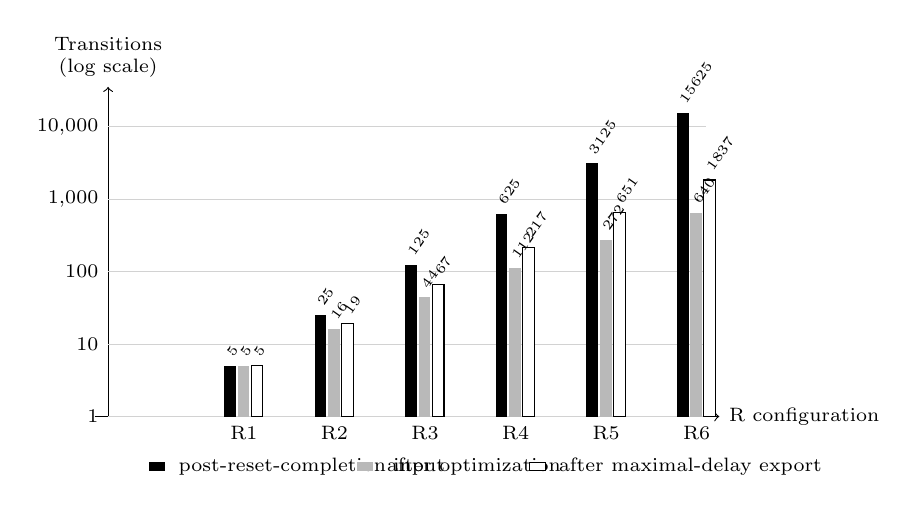
\begin{tikzpicture}[x=1.15cm,y=0.92cm,font=\scriptsize]
  % Vertical positions encode log10(edge count); the labelled y ticks are
  % 1, 10, 100, 1,000, and 10,000 transitions.
  \draw[->] (0.1,0) -- (7.0,0) node[right] {R configuration};
  \draw[->] (0.25,0) -- (0.25,4.55) node[above,align=center]
    {Transitions\\(log scale)};
  \foreach \y/\lab in {0/1,1/10,2/100,3/1{,}000,4/10{,}000} {
    \draw[gray!35] (0.25,\y) -- (6.85,\y);
    \node[left] at (0.25,\y) {\lab};
  }
  % Bars use log10(value) as height. Values above bars are exact counts.
  \foreach \x/\vin/\hin/\vopt/\hopt/\vexp/\hexp in {
    1/5/0.699/5/0.699/5/0.699,
    2/25/1.398/16/1.204/19/1.279,
    3/125/2.097/44/1.643/67/1.826,
    4/625/2.796/112/2.049/217/2.336,
    5/3125/3.494/272/2.435/651/2.814,
    6/15625/4.194/640/2.806/1837/3.264
  } {
    \pgfmathsetmacro{\xc}{\x+0.75}
    \pgfmathsetmacro{\xa}{\xc-0.22}
    \pgfmathsetmacro{\xb}{\xc-0.07}
    \pgfmathsetmacro{\xd}{\xc+0.08}
    \fill[black] (\xa,0) rectangle +(0.13,\hin);
    \fill[gray!55] (\xb,0) rectangle +(0.13,\hopt);
    \fill[white] (\xd,0) rectangle +(0.13,\hexp);
    \draw (\xd,0) rectangle +(0.13,\hexp);
    \node[rotate=55,anchor=west,font=\tiny] at (\xa,\hin+0.04) {\vin};
    \node[rotate=55,anchor=west,font=\tiny] at (\xb,\hopt+0.04) {\vopt};
    \node[rotate=55,anchor=west,font=\tiny] at (\xd,\hexp+0.04) {\vexp};
    \node[below] at (\xc,0) {R\x};
  }
  \fill[black] (0.7,-0.75) rectangle +(0.18,0.12);
  \node[right] at (0.92,-0.69) {post-reset-completion input};
  \fill[gray!55] (3.0,-0.75) rectangle +(0.18,0.12);
  \node[right] at (3.22,-0.69) {after optimization};
  \fill[white] (4.9,-0.75) rectangle +(0.18,0.12);
  \draw (4.9,-0.75) rectangle +(0.18,0.12);
  \node[right] at (5.12,-0.69) {after maximal-delay export};
\end{tikzpicture}

\caption{Post-reset-completion input, optimized TBA, and maximal-delay
explicit export for R1--R6. The logarithmic vertical axis makes the R6
concentration visible. These are the fresh five-run-median structural
counts; Comp. is the optimizer boundary, regardless of whether an upstream
Spot count happens to match it.}
\label{fig:R-transition-counts}
\end{figure*}

\subsection{Optimization effects on the generated group}
In R6, Spot emits 64 states and 15,625 cube-split transitions. The recorded
post-reset-completion optimizer input also has 64 locations and 15,625
transitions; the equality of these two edge counts is specific to R6, and the
Comp. column is the authoritative optimizer boundary. Six optimization
rounds reduce the transition relation to 640 edges and retain six clocks.
Export then produces 1,837 explicit edges, 63 invariant-bearing locations,
and 3,360 clock-difference guard occurrences; symbolic grouping represents
the output with 448 transitions. The larger explicit edge count results from
splitting disjunctive guards and adding entry conditions for invariant copies.
It measures the cost of the target representation, not a reversal of the
optimizer's reduction. In the fresh run, median optimizer and export times
are 19.812 s and 12.481 s, respectively. The October 10 and October 7 runs reported
19.345 and 13.410 s, and 25.091 and 14.572 s, with the same structural
counts; no cause for the timing changes is assigned. The generated-group table separately reports the
stage after reset completion so that upstream processing is not folded into
these optimizer measurements.

The same distinction matters for the other generated inputs. For example,
F11 starts from its actual four-location, seven-transition, two-clock TBA
after reset completion; two rounds leave the four locations and seven
transitions and remove one clock. The two locations that correspond to
states 2 and 3 of the earlier article's worked example stay separate: one
could be dropped, because $x\ge2$ always holds in the second, but location
merging requires twin transitions and their guards differ
($x\ge2\land x\le5$ against $x\le5$). N8 spends most of its end-to-end time in Spot,
whereas its recorded optimizer and exporter stages take 0.26 s and 0.68 s.
These cases show that the optimizer's cost depends on its input relation and
that the upstream producer can dominate total tool time. They do not support
a general runtime or size bound. With the tool's \texttt{-spot-level low}
option (default unchanged), N8 takes 8.9 s instead of 101.6 s, and the total
over the 29 completed configurations falls from 163 s to 46 s (one run
against the five-run medians); optimized sizes are identical except for F5
and F6 (25 to 27 symbolic transitions). R6 is dominated by the optimizer and
the export, and its faster run (32.1 s against 46.8 s) is not attributed to
the level.

\subsection{External output-size reference}
CASAAL~\cite{casaal_tool} implements the MTL$_{0,\infty}$ construction of
Li et al.~\cite{li_spin7} and prints automata with Boolean transition labels.
It is not an interchangeable optimizer: it builds its automata by its own
construction, so its sizes are a reference for the final output, not a
baseline for the optimization passes. We ran it with mutually exclusive
events, which matches the one-event-per-position words of our semantics, and
compare reachable locations and symbolic transitions of our optimized output
with CASAAL's output on the 27 configurations that both tools completed and
that CASAAL encodes exactly. The counts coincide in 24 cases. For F5 and F6
our output is larger (7 locations and 25 symbolic transitions against 4 and
15); for F14 it is smaller (6 and 14 against 8 and 18). Clock counts coincide
except for F11, where two optimization rounds reduce the two clocks of the
post-reset-completion input to one while CASAAL uses two, and F8, where the
difference comes from the upstream rewriting of $\Box\Diamond_{\ge2}p$ into
$\Box\Diamond p$ and is not credited to the optimizer. In R6 both outputs
have 64 locations and 448 symbolic transitions, whereas the optimizer input
has 15,625 explicit transitions. Whether the two tools accept the same timed
words is a question about the translation, examined in the earlier
article~\cite{fares_bodeveix_mtl_translation}; this comparison concerns sizes only.

\subsection{Matched comparison of the two export policies}
We reran R2--R6 once with each verified split policy while holding the
optimized automaton fixed. For every formula, the optimized TBA DOT files
were byte-identical across the two invocations. The table reports the
explicit-edge counts, diagonal guard atoms, and single-run exporter time
returned by the tool. Across these five inputs, all-copy export has no
explicit-edge growth beyond the optimized relation and adds no diagonal
guards. Maximal-delay export adds explicit edges in each case and introduces
2--3,360 diagonal guard atoms. This is a measured property of this benchmark
family, not a general size theorem.

\begin{table*}[t]
\centering
\caption{Matched maximal-delay and all-copy exports for R2--R6. The two
policies receive byte-identical optimized TBA graphs. Export time is one
observed run per row and policy; it is descriptive and should not be read as
a stable speed ranking.}
\label{tab:generated-export-policy}
\scriptsize
\setlength{\tabcolsep}{4pt}
\begin{tabular}{@{}lrrrrrrr@{}}
\toprule
ID & Optimized $E$ & Max-delay $E$ & All-copy $E$ & Max-delay diagonal atoms & All-copy diagonal atoms & Max-delay time (s) & All-copy time (s)\\
\midrule
R2 & 16 & 19 & 16 & 2 & 0 & 0.002 & 0.005\\
R3 & 44 & 67 & 44 & 30 & 0 & 0.014 & 0.024\\
R4 & 112 & 217 & 112 & 192 & 0 & 0.195 & 0.190\\
R5 & 272 & 651 & 272 & 880 & 0 & 1.319 & 1.052\\
R6 & 640 & 1,837 & 640 & 3,360 & 0 & 9.689 & 9.614\\
\bottomrule
\end{tabular}
\end{table*}

Both policies retain the same reachable location counts, active clock counts,
and invariant-bearing locations on these runs. Peak RSS was measured for
each full tool process, including Spot and optimization: 17.2/17.3 MB for R2
and 108.5/107.0 MB for R6 (maximal-delay/all-copy). These process-level
measurements do not isolate export memory. The observed exporter times also
have no consistent ordering: all-copy takes longer for R2/R3 and shorter for
R4/R5, with similar times for R6. The R6 policy comparison uses the same
15,625-edge post-reset-completion input and six-round, 640-edge optimized
TBA; the upstream Spot count is context, not the optimizer's pre-state.

\subsection{Translator-independent synthetic TBA suite}
To exercise the interface without the MTL translator, we construct
16 small synthetic automata directly as Rocq-representation TBA records in
\path{evaluation/synthetic_tba_bench.ml}. Their clocks are named by the six
timed subformulas of a fixed formula, the conjunction of six hatted primitive
formulas over three events; this formula is never translated and serves only
as a supply of six clock names. Locations, event labels, unary guards,
resets, and accepting locations are written by hand for each record. The suite is explicitly
synthetic: it does not parse a third-party format and is not evidence of
industrial-model performance. Its records cover redundant guards,
contradictory guards, unsatisfiable labels, a source with no incoming edge,
dead resets, synchronously reset clocks, duplicate transitions, equivalent
locations, a disjunctive-invariant export, a stable no-change input, and
targeted backward/forward propagation and pass-interaction cases.
\begin{table*}[t]
\centering
\caption{Sixteen translator-independent synthetic TBA records. Count tuples are declared locations / transitions / distinct clocks / reset occurrences / unary guard atoms; the export tuple adds diagonal guard atoms. The $I$ field gives nonempty invariant locations:bound atoms. Optimization and export times are per-call means over 200 repeated in-memory runs; RSS is the peak for a separate single-model process. Full per-pass and reachability data are supplied in the artifact.}
\label{tab:synthetic-tba}
\scriptsize
\begin{tabular}{@{}lrrrrrrr@{}}
\toprule
Model & Input & Optimized & Rounds & Opt. (ms) & RSS (KiB) & Export & Exp. (ms)\\
\midrule
stable & 1/1/0/0/0 & 1/1/0/0/0; $I=0:0$ & 0 & 0.008 & 6364 & 2/1/0/0/0/0; $I=1:0$ & 0.089\\
redundant\_guard & 2/2/1/1/3 & 2/2/1/1/2; $I=2:2$ & 1 & 0.133 & 6460 & 4/2/1/1/2/0; $I=2:2$ & 0.197\\
contradictory\_guard & 2/2/1/0/2 & 2/1/0/0/0; $I=0:0$ & 1 & 0.042 & 6428 & 4/1/0/0/0/0; $I=1:0$ & 0.073\\
unsatisfiable\_label & 2/2/0/0/0 & 2/1/0/0/0; $I=0:0$ & 1 & 0.026 & 6352 & 4/1/0/0/0/0; $I=1:0$ & 0.143\\
isolated\_source & 3/2/0/0/0 & 3/1/0/0/0; $I=0:0$ & 1 & 0.027 & 6340 & 6/1/0/0/0/0; $I=1:0$ & 0.264\\
dead\_reset & 2/2/1/2/0 & 2/2/0/0/0; $I=0:0$ & 1 & 0.052 & 6468 & 4/2/0/0/0/0; $I=2:0$ & 0.150\\
normalization\_dead\_reset & 2/2/1/1/1 & 2/2/0/0/0; $I=0:0$ & 1 & 0.110 & 6336 & 4/2/0/0/0/0; $I=2:0$ & 0.491\\
synchronous\_clock\_merge & 2/3/2/2/2 & 2/3/1/1/2; $I=1:1$ & 2 & 0.673 & 6300 & 4/3/1/1/2/0; $I=2:1$ & 1.279\\
duplicate\_transition & 2/3/1/2/3 & 2/2/1/1/2; $I=2:2$ & 1 & 0.267 & 6364 & 4/2/1/1/2/0; $I=2:2$ & 0.478\\
equivalent\_locations & 3/4/0/0/0 & 3/2/0/0/0; $I=0:0$ & 2 & 0.104 & 6404 & 6/2/0/0/0/0; $I=2:0$ & 0.220\\
disjunctive\_invariant\_export & 3/3/2/0/2 & 3/3/2/0/2; $I=0:0$ & 0 & 0.095 & 6488 & 9/6/2/0/12/6; $I=3:2$ & 1.154\\
backward\_tightening & 2/2/1/0/2 & 2/2/1/0/2; $I=2:2$ & 1 & 0.093 & 6360 & 4/2/1/0/2/0; $I=2:2$ & 0.204\\
forward\_lower\_bound & 3/3/1/0/2 & 3/3/1/0/4; $I=2:2$ & 1 & 0.141 & 6460 & 6/3/1/0/4/0; $I=3:2$ & 0.654\\
forward\_contradiction\_cascade & 6/7/1/0/3 & 6/4/1/0/4; $I=1:1$ & 2 & 0.437 & 6428 & 12/4/1/0/4/0; $I=3:1$ & 1.082\\
backward\_contradiction\_cascade & 5/5/1/0/4 & 5/1/0/0/0; $I=0:0$ & 2 & 0.201 & 6320 & 10/1/0/0/0/0; $I=1:0$ & 0.180\\
clock\_merge\_contradiction\_cascade & 5/5/2/6/4 & 5/3/1/2/1; $I=1:1$ & 2 & 0.622 & 6484 & 10/2/1/2/1/0; $I=2:1$ & 0.598\\
\bottomrule
\end{tabular}
\end{table*}


The harness reports counts after every pass in every round and checks that
its profiled pass sequence is structurally equal to the extracted
\texttt{optimize\_step} on each round. It also times the unprofiled iterative
optimizer and export as means over 200 repeated in-memory calls per model.
Standalone process RSS ranges from 6,184 to 6,484 KiB. These short timings
and small, purpose-built records are microbenchmark evidence only; the raw
pass table and per-model RSS file are supplied for reproduction. Per-pass
times are recorded but are too small to support fine-grained speed rankings.

The targeted examples exercise both bound-propagation directions. Backward
synthesis tightens an incoming $x\leq5$ guard to $x\leq2$. Forward
propagation adds an entry lower bound $x\geq2$ to outgoing edges. In the
forward-cascade input, an alternate $x\leq10$ branch prevents backward
synthesis from creating the contradiction; forward propagation makes the
$x\leq1$ branch contradictory, and the following pruning stages remove its
unentered chain. Omitting forward propagation retains all seven input edges,
while the full optimizer leaves four. A separate backward cascade isolates
that pass. Table~\ref{tab:synthetic-interactions} shows input/output counts
and leave-one-operation-out effects.

The normalization/reset example removes a tautological $x\geq0$ guard before
dead-reset analysis, allowing its reset and active clock to be removed. The
synchronous-clock example first merges the clocks, then a later round detects
the conflicting $x\geq5\land x\leq3$ guard and prunes the branch. Other
records measure unsatisfiable-label elimination, no-incoming-source pruning,
transition subsumption, and equivalent-location merging. The no-incoming
operation is a local predecessor test, not full graph reachability. These
interactions explain the iterative design; preservation for each finite
iteration count follows from the proved pass composition.
\begin{table*}[t]
\centering
\caption{Measured direct TBA examples targeting propagation and pass interactions. Transition and clock counts are total records and active clocks. Leave-one-operation-out variants are experimental composites, not separately verified transformations.}
\label{tab:synthetic-interactions}
\scriptsize
\setlength{\tabcolsep}{3pt}
\begin{tabular}{@{}p{0.22\textwidth}cccp{0.39\textwidth}@{}}
\toprule
Case & Input $E/C$ & Full $E/C$ & Rounds & Measured target-pass effect when omitted\\
\midrule
Backward bound tightening & 2/1 & 2/1 & 1 & Incoming guard tightens from $x\leq5$ to $x\leq2$; omitting backward synthesis leaves $x\leq5$.\\
Forward lower-bound propagation & 3/1 & 3/1 & 1 & Entry fact $x\geq2$ is added to the outgoing $q$ edge; edge count is unchanged.\\
Forward contradiction cascade & 7/1 & 4/1 & 2 & Omitting forward propagation or contradiction removal retains 7 edges; the full run removes the $x\leq1$ branch and then prunes its unentered chain.\\
Backward contradiction cascade & 5/1 & 1/0 & 2 & Omitting backward synthesis leaves 2 edges/1 clock; omitting contradiction removal leaves 5/1.\\
Normalization and dead reset & 2/1 & 2/0 & 1 & Normalizing tautological $x\geq0$ enables reset removal; omitting either pass leaves 1 active clock.\\
Synchronous-clock contradiction & 5/2 & 3/1 & 2 & Merging the synchronously reset clocks exposes $x\geq5\land x\leq3$; omitting clock merge or contradiction removal leaves 5 edges/2 clocks.\\
\bottomrule
\end{tabular}
\end{table*}


Table~\ref{tab:synchronous-trace} gives the measured stage interaction for
the largest synchronously reset synthetic input. Unsatisfiable-label removal
first reduces the relation from seven edges to five. Dead-reset elimination
then lowers the active-clock count from six to four. The synchronous-clock
pass changes the synthesized invariant, and the next round's dead-reset pass
removes the remaining redundant resets, leaving one active clock. This is a
measurement of the extracted implementation; the language-preservation
claim follows separately from the proved pass composition.
\begin{table*}[t]
\centering
\caption{Measured trace for the six-clock synchronous-reset synthetic input. Counts are declared / reachable locations, transitions, active clocks, reset occurrences, guard atoms, invariant locations / atoms, and diagonal guard atoms. The export row is the internal explicit DTA.}
\label{tab:synchronous-trace}
\scriptsize
\setlength{\tabcolsep}{3pt}
\begin{tabular}{@{}p{0.27\textwidth}rrrrrrr@{}}
\toprule
Stage & $L/R$ & $E$ & $C$ & Resets & Guard atoms & Inv. $L/A$ & Diag.\\
\midrule
Input & 2/2 & 7 & 6 & 6 & 6 & 0/0 & 0 \\
R1: unsatisfiable-label removal & 2/2 & 5 & 6 & 6 & 4 & 0/0 & 0 \\
R1: dead-reset elimination & 2/2 & 5 & 4 & 4 & 4 & 0/0 & 0 \\
R1: synchronous-clock pass & 2/2 & 5 & 4 & 4 & 4 & 1/1 & 0 \\
R2: dead-reset elimination & 2/2 & 5 & 1 & 1 & 4 & 1/1 & 0 \\
Optimized fixed point & 2/2 & 5 & 1 & 1 & 4 & 1/1 & 0 \\
Explicit export & 4/2 & 5 & 1 & 1 & 4 & 2/1 & 0 \\
\bottomrule
\end{tabular}
\end{table*}


The synthetic disjunctive-invariant case is unchanged by optimization, then
grows from three locations and three transitions to nine locations and six
explicit transitions after export. The output has conjunctive invariants and
six diagonal guard atoms that select maximal-delay copies. This is a
measured size cost of export; the output-shape guarantee itself follows from
\texttt{export\_guards\_conjunctive} and
\texttt{export\_invariants\_conjunctive}.

\subsection{Pass ablation and parameterized synthetic families}
To measure pass interactions, we repeated the same composite pipeline while
omitting one operation at a time from sixteen fixed synthetic input records. Each
modified composite was iterated to structural stability (at most 50 changed
rounds); this is a measurement driver, not a separate Rocq theorem about the
ablated variants. The full variant was checked for structural equality with
the extracted optimizer on each input. Table~\ref{tab:synthetic-ablation}
reports aggregate reachable locations, total transition records, active
clocks, changed rounds, and median repeated-call time. The raw TSV gives each
record and its counts under every pass.

The aggregate ablation shows effects that selected records were designed to
expose. Relative to the full variant (33 transitions and nine active clocks
summed across the suite), omitting backward synthesis leaves 34 transitions
and ten clocks; omitting forward propagation leaves 36 transitions; and
omitting contradiction removal leaves 43 transitions. Omitting pruning of
sources without incoming edges leaves 39 transitions. Normalization and
dead-reset omission raise the aggregate active-clock count to 12 and 13,
respectively. Omitting synchronous-clock merging leaves 35 edges and 11
clocks; omitting transition merging leaves 35 edges, while omitting
equivalent-location merging leaves one more reachable location. These are
descriptive differences on a deliberately selected synthetic suite, not
estimates of typical pass effects. Per-call medians are too small for
fine-grained pass runtime rankings; process RSS includes runtime overhead.
\begin{table*}[t]
\centering
\caption{Iterated leave-one-operation-out ablations on sixteen fixed synthetic TBA records. Reachable-location, transition, and active-clock counts are summed across the same inputs; rounds and runtime are medians across inputs. Runtime is the median of each model's mean over 200 in-memory runs. Each variant repeats its retained composite to structural stability. The full variant is checked against the extracted optimizer; the modified ablation driver is not a separate Rocq theorem.}
\label{tab:synthetic-ablation}
\scriptsize
\setlength{\tabcolsep}{3pt}
\begin{tabular}{@{}p{0.32\textwidth}rrrrrr@{}}
\toprule
Variant & $\sum L_{\rm reach}$ & $\sum E$ & $\sum C$ & med. rounds & med. time (ms) & cases with $E$ above full\\
\midrule
Full optimizer & 30 & 33 & 9 & 1 & 0.102 & 0 \\
Omit bound synthesis/backward propagation & 31 & 34 & 10 & 1 & 0.104 & 1 \\
Omit forward propagation & 33 & 36 & 9 & 1 & 0.085 & 1 \\
Omit contradictory-edge removal & 40 & 43 & 11 & 1 & 0.102 & 4 \\
Omit unsatisfiable-label removal & 31 & 34 & 9 & 1 & 0.105 & 1 \\
Omit no-incoming-source pruning & 30 & 39 & 10 & 1 & 0.098 & 4 \\
Omit guard normalization & 30 & 33 & 12 & 1 & 0.107 & 0 \\
Omit dead-reset removal & 30 & 33 & 13 & 1 & 0.101 & 0 \\
Omit synchronous-clock merging & 32 & 35 & 11 & 1 & 0.091 & 1 \\
Omit transition merging & 30 & 35 & 9 & 1 & 0.084 & 2 \\
Omit equivalent-location merging & 31 & 35 & 9 & 1 & 0.068 & 1 \\
\bottomrule
\end{tabular}
\end{table*}


We also constructed five size-parameterized families directly in the formal
TBA representation, without a third-party parser. Table~\ref{tab:parameterized-synthetic}
reports every tested size. In the duplicate-edge family, inputs grow from
two to 33 edges while optimization reduces each nontrivial instance to two.
The unreachable-cascade sweep includes sizes 1--50, 51, and 64; rows at the
50-round driver cap are marked and report capped, not necessarily stable,
outputs. A separate probe confirms that size 51 still changes on round 51
(two edges remain after round 50), while size 64 still changes on rounds 51
and 52. The size-50 chain has one edge after round 50 and is unchanged by
round 51, but the driver conservatively warns because it did not perform that
stability check. Synchronously reset families with two to six clocks reduce
to one active clock in two rounds.
The disjunctive-invariant export grows from 10 edges and 10 diagonal guard
occurrences at $k=2$ to 68 edges and 204 diagonal occurrences at $k=6$.
These counts expose representation costs in a deliberately constructed
stress family; they are not industrial-model measurements or a complexity
bound. For every finite number of rounds, including a capped result,
\texttt{optimize\_accepts} preserves language. Reaching the iteration cap
does not justify calling that result a fixed point. Per-size intermediate
records and the exact cap probe are preserved in the dated run artifacts.
\begin{table*}[t]
\centering
\caption{Complete parameter sweeps for five translator-independent synthetic TBA families. Tuples report declared locations / graph-reachable locations / transitions / active clocks. The optimizer count is the number of structurally changed rounds; optimization time is the mean over 200 in-memory calls. Export diagonals are explicit clock-difference guard occurrences.}
\label{tab:parameterized-synthetic}
\scriptsize
\setlength{\tabcolsep}{2.5pt}
\begin{tabular}{@{}p{0.19\textwidth}r p{0.16\textwidth}p{0.16\textwidth}r p{0.16\textwidth}rr@{}}
\toprule
Family & $k$ & Input $L/R/E/C$ & Opt. $L/R/E/C$ & Rnds. & Export $L/R/E/C$ & Opt. (ms) & Diag.\\
\midrule
Duplicate edges & 1 & 2/2/2/0 & 2/2/2/0 & 0 & 4/2/2/0 & 0.017 & 0 \\
Duplicate edges & 2 & 2/2/3/0 & 2/2/2/0 & 1 & 4/2/2/0 & 0.030 & 0 \\
Duplicate edges & 4 & 2/2/5/0 & 2/2/2/0 & 1 & 4/2/2/0 & 0.046 & 0 \\
Duplicate edges & 8 & 2/2/9/0 & 2/2/2/0 & 1 & 4/2/2/0 & 0.057 & 0 \\
Duplicate edges & 16 & 2/2/17/0 & 2/2/2/0 & 1 & 4/2/2/0 & 0.073 & 0 \\
Duplicate edges & 32 & 2/2/33/0 & 2/2/2/0 & 1 & 4/2/2/0 & 0.216 & 0 \\
Unreachable cascade & 1 & 3/1/2/0 & 3/1/1/0 & 1 & 6/1/1/0 & 0.027 & 0 \\
Unreachable cascade & 2 & 4/1/3/0 & 4/1/1/0 & 2 & 8/1/1/0 & 0.075 & 0 \\
Unreachable cascade & 4 & 6/1/5/0 & 6/1/1/0 & 4 & 12/1/1/0 & 0.253 & 0 \\
Unreachable cascade & 8 & 10/1/9/0 & 10/1/1/0 & 8 & 20/1/1/0 & 1.752 & 0 \\
Unreachable cascade & 16 & 18/1/17/0 & 18/1/1/0 & 16 & 36/1/1/0 & 9.324 & 0 \\
Unreachable cascade & 32 & 34/1/33/0 & 34/1/1/0 & 32 & 68/1/1/0 & 47.381 & 0 \\
Unreachable cascade & 50 & 52/1/51/0 & 52/1/1/0 & 50 & 104/1/1/0 & 227.747 & 0 \\
Unreachable cascade & 51 & 53/1/52/0 & 53/1/2/0 & 50 & 106/1/1/0 & 239.316 & 0 \\
Unreachable cascade & 64 & 66/1/65/0 & 66/1/15/0 & 50 & 132/1/1/0 & 531.813 & 0 \\
Redundant bounds & 1 & 2/2/2/1 & 2/2/2/1 & 0 & 4/2/2/1 & 0.017 & 0 \\
Redundant bounds & 2 & 2/2/2/1 & 2/2/2/1 & 1 & 4/2/2/1 & 0.025 & 0 \\
Redundant bounds & 4 & 2/2/2/1 & 2/2/2/1 & 1 & 4/2/2/1 & 0.027 & 0 \\
Redundant bounds & 8 & 2/2/2/1 & 2/2/2/1 & 1 & 4/2/2/1 & 0.036 & 0 \\
Redundant bounds & 16 & 2/2/2/1 & 2/2/2/1 & 1 & 4/2/2/1 & 0.034 & 0 \\
Synchronous resets & 2 & 2/2/3/2 & 2/2/3/1 & 2 & 4/2/3/1 & 0.230 & 0 \\
Synchronous resets & 3 & 2/2/4/3 & 2/2/4/1 & 2 & 4/2/4/1 & 0.316 & 0 \\
Synchronous resets & 4 & 2/2/5/4 & 2/2/4/1 & 2 & 4/2/4/1 & 0.318 & 0 \\
Synchronous resets & 6 & 2/2/7/6 & 2/2/5/1 & 2 & 4/2/5/1 & 0.618 & 0 \\
Disjunctive invariant & 2 & 2/2/3/2 & 2/2/3/2 & 0 & 6/3/10/2 & 0.030 & 10 \\
Disjunctive invariant & 3 & 2/2/4/3 & 2/2/4/3 & 0 & 8/4/30/3 & 0.047 & 60 \\
Disjunctive invariant & 4 & 2/2/5/4 & 2/2/4/3 & 1 & 8/4/30/3 & 0.117 & 60 \\
Disjunctive invariant & 6 & 2/2/7/6 & 2/2/5/4 & 1 & 10/5/68/4 & 0.213 & 204 \\
\bottomrule
\end{tabular}
\end{table*}


\subsection{UPPAAL and timed-liveness checks}
The four UPPAAL configurations are two parameterized system families: a
sporadic emitter with minimum separation two (satisfying) or one (violating),
and a request/response controller with response bound four (satisfying) or
six (violating). The property query reaches a designated violation sink; it
does not ask UPPAAL to check B\"uchi acceptance.
\begin{table*}[t]
\centering
\caption{UPPAAL safety-query results for the two packaged system families. The queries were rerun with the UPPAAL 5.0.0 verifier (\texttt{verifyta}) on the packaged models; the verdicts are identical to the earlier archived ones.}
\label{tab:uppaal-results}
\scriptsize
\begin{tabular}{@{}lllc@{}}
\toprule
Family & Configuration & Query & Verdict\\
\midrule
Sporadic emitter & Minimum separation $2$ & \texttt{E<> P.A4} & Not satisfied (expected)\\
Sporadic emitter & Minimum separation $1$ & \texttt{E<> P.A4} & Satisfied (violation trace)\\
Request/response & Response bound $4$ & \texttt{E<> P.A4} & Not satisfied (expected)\\
Request/response & Response bound $6$ & \texttt{E<> P.A4} & Satisfied (violation trace)\\
\bottomrule
\end{tabular}
\end{table*}
The system-only \texttt{A[] not deadlock} query is satisfied for
all four models; that result does not establish time divergence. The packaged
traces show the violating event pairs. The result files contain verdicts and
traces, not before/after optimization runtimes, memory, zone, or state counts,
so they demonstrate use of the exported models rather than a quantified
model-checking speedup.

The eight queries (four reachability, four deadlock) were rerun with
UPPAAL 5.0.0 (revision 714BA9DB36F49691, June 2023) on the packaged models;
all eight verdicts coincide with the archived ones.

For liveness, we reran the separate TChecker timed B\"uchi emptiness case and
added a matched before/after comparison. Before uses zero optimizer rounds;
after requests the tool's 50-round maximum. Both formula-generated outputs
satisfy \texttt{init\_free}=1, so their zero clock initialization matches the
TChecker product's zero-start convention for these cases. The system template
was extracted from the archived UPPAAL model by the unverified
\texttt{tck\_normalize\_system.py} adapter. The same system, property
automaton, event synchronization, strict timestamp process, time-divergence
process, and TChecker settings were used on both sides.

\begin{table*}[t]
\centering
\caption{Matched TChecker timed-B\"uchi emptiness before and after the optimizer. State counts are stored/visited; runtime is the checker's reported time and peak RSS is the whole TChecker process. The exported XML and product automata are byte-identical within each pair.}
\label{tab:tchecker-before-after}
\scriptsize
\begin{tabular}{@{}lccccc@{}}
\toprule
System & \texttt{CYCLE} before/after & Stored/visited states before/after & Visited transitions & Runtime before/after (ms) & Peak RSS before/after (KiB)\\
\midrule
Responds within 4 units & false / false & 77/77 / 77/77 & 127/127 & 0.542 / 0.844 & 8,136 / 8,144\\
May remain busy forever & true / true & 15/7 / 15/7 & 19/19 & 0.138 / 0.105 & 8,120 / 8,016\\
\bottomrule
\end{tabular}
\end{table*}

In both pairs the after run reported one changed optimizer round, but its
exported XML hash matched the before XML, and the generated TChecker products
were byte-identical. The checker explored the same states and transitions
and returned the same verdict. These measurements show no downstream
structural or exploration change for these examples; they do not demonstrate
a speedup or a regression. TChecker checks nonemptiness of a timed-B\"uchi
product over strictly increasing, time-divergent words. This remains distinct
from UPPAAL's ordinary reachability and deadlock queries. Checker verdicts
are experiments, not Rocq proofs. XML printing, the adapter, and format
correspondence remain outside the mechanized interface; Rocq proves shape
properties only for the internal DTA.

\subsection{Limitations}
The generated benchmark uses one upstream toolchain and the independent
suite uses deliberately small synthetic inputs. The independent synthetic
families demonstrate direct applicability to selected input shapes,
but do not establish broad empirical support for arbitrary automata. No
verified third-party parser or broad external TBA corpus is included. Export can grow both the
state and transition representations. The matched TChecker study is limited
to two response-system cases whose exported products were identical, and
therefore gives no evidence of a performance benefit. Performance conclusions are limited to
these measured inputs. The preservation theorems are universal only over the
formal Rocq TBA interface and its timed-word semantics; that scope does not
extend through an unverified adapter to arbitrary file formats.
